\documentclass[border=10pt]{standalone}
\usepackage{pgfplots}
\usepgfplotslibrary{colormaps}
\pgfplotsset{compat=1.18}

\begin{document}
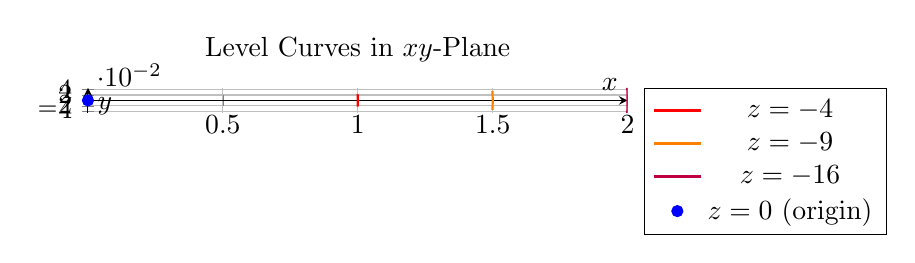
\begin{tikzpicture}
\begin{axis}[
    xlabel={$x$},
    ylabel={$y$},
    title={Level Curves in $xy$-Plane},
    domain=-2:2,
    samples=50,
    axis lines=center,
    grid=major,
    axis equal image,
    legend pos=outer north east,
]
% Ellipse at z = -4: x^2/1 + y^2/(4/9) = 1
\addplot[thick, red] ({cos(\x)}, {(2/3)*sin(\x)});

% Ellipse at z = -9: x^2/(9/4) + y^2/1 = 1
\addplot[thick, orange] ({1.5*cos(\x)}, {sin(\x)});

% Ellipse at z = -16: x^2/4 + y^2/(16/9) = 1
\addplot[thick, purple] ({2*cos(\x)}, {(4/3)*sin(\x)});

% Point at z = 0
\addplot[only marks, mark=*, blue] coordinates {(0,0)};

\legend{$z=-4$, $z=-9$, $z=-16$, $z=0$ (origin)}
\end{axis}
\end{tikzpicture}
\end{document}
